\documentclass{scrreprt}
\usepackage[utf8]{inputenc}
\usepackage{lmodern}
\usepackage{listings}
\usepackage{underscore}
\usepackage{graphicx}
\usepackage[margin=0.5in]{geometry}
\usepackage[bookmarks=true]{hyperref}
\hypersetup{
    bookmarks=false,    % show bookmarks bar?
    colorlinks=true,       % false: boxed links; true: colored links
    linkcolor=blue,       % color of internal links
    citecolor=black,       % color of links to bibliography
    filecolor=black,        % color of file links
    urlcolor=purple,        % color of external links
    linktoc=page            % only page is linked
}%
\def\myversion{1.0 }
\title{%
\flushleft
\rule{16cm}{5pt}\vskip1cm
\Huge{DESIGN SPECIFICATION}\\
for\\
Pok\'eSnowdown \\
\vspace{2cm}
\LARGE{Version \myversion\\}
\vspace{2cm}
Produced by Matthew Zang, Nicholas Cage, Chiraq Obama, 4Evar Young\\
\vfill
\rule{16cm}{5pt}
}

\date{}
\usepackage{hyperref}
\begin{document}
\newgeometry{left=3cm,bottom=0.1cm}
\maketitle
\tableofcontents
\restoregeometry
\chapter*{Update Log}

This log will hold all the updates/git pushes to our game, showing our current progress/what needs to be completed, etc...

\chapter{System Description}
\section{Core Vision}

Our plan for A6 is to create a Pok\'emon Showdown spinoff using \texttt{OCaml} using key concepts presented in class (concurrency, mutability, functional programming) as well as integrating functions of \texttt{OCaml} not presented in class, including producing a suitable GUI and server to aid in development of the game. To set us apart from Pok\'emon Showdown, we are incorporating a single-player story mode in the form of a "Tournament mode", as well as allowing for full 1-Player, 2-Player, and No-Player functionality (by developing an intelligent bot that can fully play the game).

\section{Key Features}
We hope to have the following implemented in our completed project:
\begin{enumerate}
	\item A fully functional GUI that allows the players to see the current state of the game. The GUI will most likely show the Pok\'emon but the attack animations might be too complex to complete. 
	\item All the current Pok\'emon will be included in the game, as well as items that are commonly used in competitive battling will also be included.
	\item Multiple game options. We are hoping to have the following modes.
		\begin{itemize}
			\item For 1-Player, we hope to incorporate three different modes. 
				\begin{enumerate}
					\item \textbf{Random Battles}: This is the same game mode as commonly found on Pok\'emon Showdown where teams are randomized. However, the player will be playing against the AI.
					\item \textbf{Tournament mode}: This is the single player story mode that we plan on incorporating.
					\item \textbf{Preset Battles}: The player gets to create his own Pok\'emon team and play against AI that use pre-made Smogon team compositions.
				\end{enumerate}
			\item For 2-Player, we hope to have a single game mode.
				\begin{enumerate}
					\item \textbf{Friend Battles}: Players have the options of choosing a Random team or a Preset team to head into battle with their friend.
				\end{enumerate}
			\item Lastly, for No-Player, we hope to have a single game mode.
				\begin{enumerate}
					\item \textbf{SkyNet Battles}: Player has option of choosing the Pok\'emon team for two bots, and watch them as they face off.
				\end{enumerate}
		\end{itemize}
	\item We wish to provide a Pok\'emon team editor that allows a player to choose Pok\'emon and movesets. This team is saved and can be loaded up for future use. These teams will be used in the game modes described above.
	\item We wish to integrate mustic into our game based upon the game mode as well as the current battle status.
	\item We want to include an interactive story mode/dialogue that will describe the underlying storyline in our Tournament mode. 
	\item We will have to include concurrency for two player battling, meaning that there will have to be a server to respond to player requests as well as the GUI. 
\end{enumerate}

\section{Narrative Description}
	This game will be an upgraded version of Pok\'emon Showdown, suitable and to the scale for a small console video game. It will have the main aspects of Pok\'emon Showdown including random battles between two players, as well as premade team battles between two players and a fully functional Pok\'emon team editor. However, it will also include single player capabilities, such as random battling or premade battling against an AI. The AI must be able to battle effectively and use advanced Pok\'emon techniques in the battle. In addition to this, there will be a Tournament mode which is essentially a story mode. The player has to play against several bots before proceeding to the final boss. This means that bots should have different levels of intelligence in order for this game mode to be challenging. 
\chapter{Architecture}
	We are aiming to produce a client-server architecture. The game server will keep track of the current game state, make sure all the rules of Pok\'emon are followed, update the GUI, etc... while the client (the players) send messages to the server to retrieve information as well as request to perform certain game actions. There will be at most three clients (the GUI that displays the current state of the game, and the other two clients are the players). When the game is launched, it waits until it establishes a connection with the GUI through a different port allowing multiple people to watch instances of their own GUI. Then it spawns a thread while waiting for either two players (either real players or AI to connect). It initializes the players and then starts the game. The C\&C diagram is shown below. 
	
	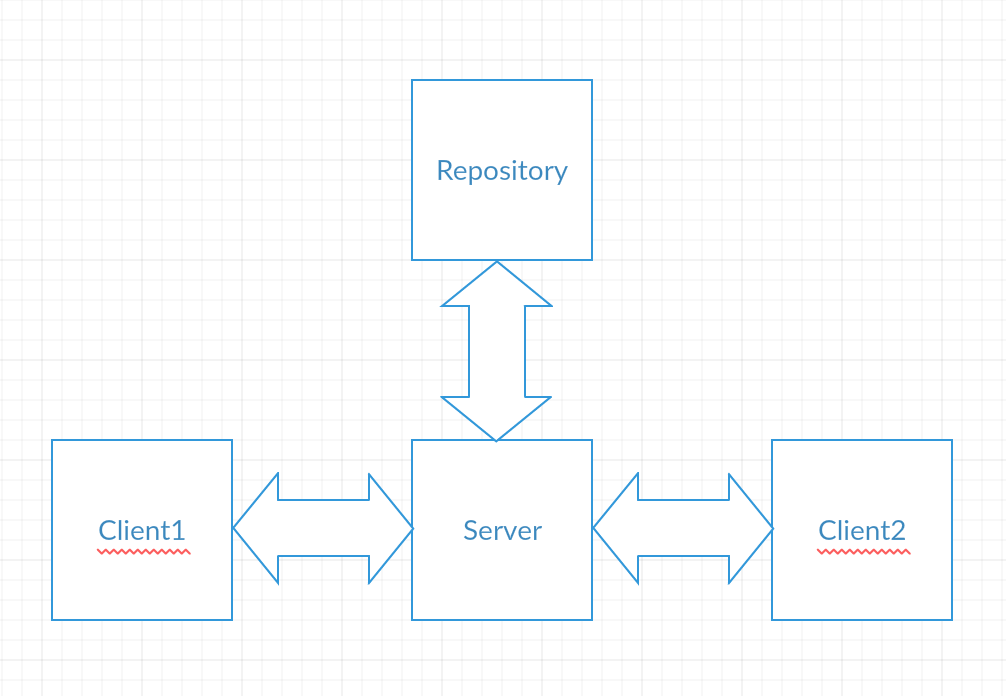
\includegraphics{C&C.png}

\chapter{System Design}
\section{Important Modules}

\begin{enumerate}
	\item Game.ml
\end{enumerate}
\chapter{Module Design}
\chapter{Data}
\chapter{External Dependencies}
\chapter{Testing Plan}

% add other chapters and sections to suit
\end{document}